\section{What did not transfer: five reconstructions}\label{app:reconstructions}

We reconstructed five recent approaches in an open-source stack (Python 3.12, SCIP 10 via
PySCIPOpt 6.2, HiGHS 1.15, OR-Tools 9.15, PyTorch on CPU). These are methodological
reconstructions: the original code requires historical environments or commercial licenses, and
no original number is claimed as reproduced. Each was compared with the classical rule that
performs the same function.

\begin{table}[h]\centering\small
\caption{Reconstructions and their classical counterparts.}\label{tab:recon}
\begin{tabular}{p{3.0cm}p{4.3cm}p{6.2cm}}
\toprule
Approach & What the learned component does & Outcome against the classical counterpart \\
\midrule
Learned branching \citep{gasse2019,gupta2020} & ranks branching candidates by imitating strong
branching (953 samples) & on 20 \texttt{facilities} instances (100$\times$100), 91.7~s vs.\
100.1~s for reliability pseudocost (shifted geometric means), but with 167 vs.\ 49 nodes and on
par with plain pseudocost (93.2~s); top-1 accuracy equal to most-fractional (0.36 vs.\ 0.39) \\
Learned swap filters \citep{guo2023swap,su2024urban} & selects which swaps of a $p$-median local
search to evaluate & without fallback, the classical add-gain filter gave 47$\times$ speedup with
6.6\% loss at $n=1000$; the learned filter gave 14$\times$ with 8.8\% and won only at the training
scale ($n=200$) \\
Unsupervised MPNN for uniform facility location \citep{qian2026unifl} & predicts opening
probabilities trained on an expected-cost loss & after stabilizing training (3 of 4 seeds
collapsed in the pre-registered version), 1.026 of the best known at $n=1000$ vs.\ 1.186 for
Mettu--Plaxton; with local search both are within 0.6\% of the optimum \\
Neural embedded MIP for location-routing \citep{kaleem2024neo} & a Deep Sets routing-cost
surrogate embedded in the location MIP & with big-M ReLU encodings in SCIP the MIP never left its
initial solution (dual gap 591\% after 120~s); a linear continuous approximation had median
deviation 0.03\% vs.\ 0.05--0.30\% for the neural variants \\
Learned pruning (this paper, Section~\ref{sec:res-pruning}) & keeps the top-ranked facilities &
the LP ranking matched or beat the GNN except at 80\% kept facilities \\
\bottomrule
\end{tabular}
\end{table}

\begin{figure}[h]\centering
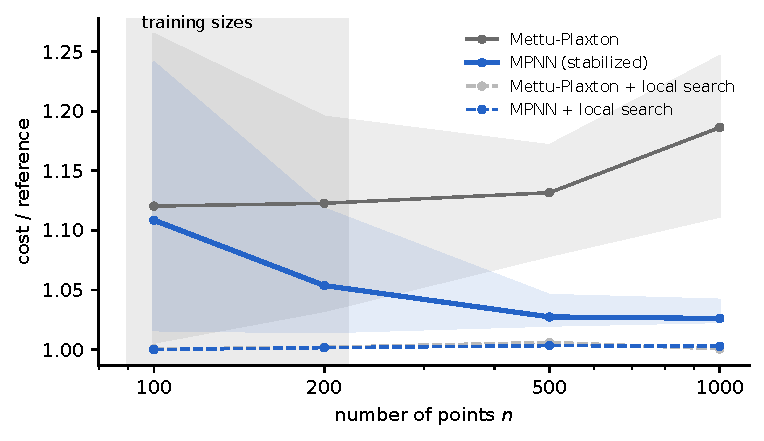
\includegraphics[width=0.85\linewidth]{../figuras/unifl.pdf}
\caption{Uniform facility location: cost of each method divided by a reference, as a function of
the number of points $n$ (log scale). The reference is the optimum proven by SCIP for $n\le 500$
(time limit 120--300~s) and the best solution found by any method for $n=1000$. A ratio of 1.00
is optimal; 1.10 is 10\% above. Lines are medians over the test instances (20, 20, 10 and 6 for
$n=100, 200, 500, 1000$); shaded bands are the 10th--90th percentiles, drawn only for the methods
without local search. \emph{Mettu--Plaxton}: the radius-based 3-approximation. \emph{MPNN
(stabilized)}: message-passing network trained without labels on an expected-cost loss, with
output probabilities clipped to $[0.01, 0.99]$ and gradient clipping (two seeds); the
pre-registered version collapsed in 3 of 4 seeds. Dashed lines add an add/drop/swap local search
to each. The grey band marks the sizes used for training. Source:
\texttt{results/pesquisa/unifl/}.}
\label{fig:unifl}
\end{figure}

\begin{figure}[h]\centering
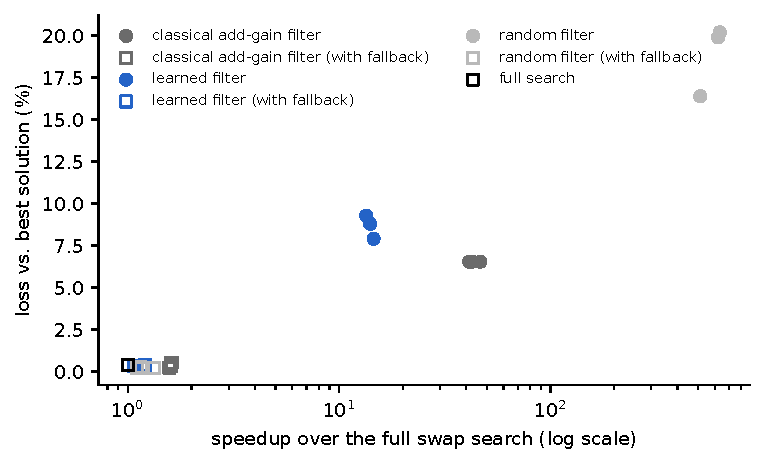
\includegraphics[width=0.85\linewidth]{../figuras/trocas.pdf}
\caption{Swap filters for the weighted $p$-median on synthetic road networks with $n=1000$ nodes
(5 networks, 3 random starts each). Each point is one filter configuration (8, 16 or 32 entering
candidates evaluated per iteration); coordinates are medians over the 15 runs. \emph{Horizontal
axis}: speedup, the running time of the full swap search divided by the running time of the
filtered search from the same start (log scale; 10 means ten times faster). \emph{Vertical axis}:
loss, the final cost relative to the best solution found by any configuration, in percent.
Filled circles stop when no filtered swap improves (the regime of the original papers); hollow
squares run one full sweep before stopping, which guarantees a true local optimum of the full
neighborhood. \emph{Classical add-gain filter}: ranks entering facilities by
$\sum_j w_j \max(0, d^{(1)}_j - d_{kj})$ and leaving facilities by their removal loss.
\emph{Learned filter}: two gradient-boosted regressors imitating the best exact swap gain, trained
on networks with $n=200$. Source: \texttt{results/pesquisa/swap\_v2/}.}
\label{fig:swaps}
\end{figure}

The common pattern is that the speedups reported for learned components often come from the
mechanism the learning plugs into (filtering candidate moves, decomposing the problem, embedding
a cheaper objective) rather than from the learning itself, which is why the classical
counterpart, given the same budget, is the necessary baseline.
